\documentclass{beamer}
\usepackage[polish,british]{babel}
\usepackage[utf8]{inputenc}
\usepackage{enumerate}
\usepackage{tabu}
\setbeamertemplate{itemize item}[square]
\setbeamertemplate{itemize subitem}[circle]

\author{Paweł Paczuski }
\title{Structured radiological reporting system}
\date{29.06.2018}
\begin{document}
\begin{frame}
\titlepage
\end{frame}


\section{Introduction}
\subsection{Problems of modern medicine}
\begin{frame}
\frametitle{Areas of interest of modern medicine}
\begin{itemize}
	\item increasing variety of diagnostic techniques and procedures
	\item unsatisfiable demand for medical services
	\item bureaucracy
	\item clinical data and reporting (store and exchange)
\end{itemize}
\end{frame}


\subsection{Standards}
\subsection{Typical workflow of a radiologist}
\begin{frame}
\frametitle{Typical workflow of a radiologist}
\begin{figure}
	\centering
	\includegraphics[width=1\linewidth]{../workspace}
	\caption{Typically, a radiologist analyzes medical images and creates report's text simultaneously}
	\label{fig:workspace}
\end{figure}
\end{frame}

\begin{frame}
\frametitle{Areas where productivity optimizations could be applied}
What can be improved:
\begin{itemize}
	\item radiologists are \alert{very BAD} at typing on keyboard
	\item speech recognition has problems with capturing medical language
	\item reporting quality  
\end{itemize}

How:
\begin{itemize}
	\item typing on keyboard replaced by checking boxes with predefined phrases
	\item reports represented as trees that have relations between causes and effects
	\item workflow organized around set of checklists and \alert{templates}
\end{itemize}
\end{frame}


\section{Design and implementation of Structured reporting system}
\subsection{Radiological report as a tree}


\begin{frame}
\frametitle{Radiological report as a tree}
\begin{figure}
	\centering
	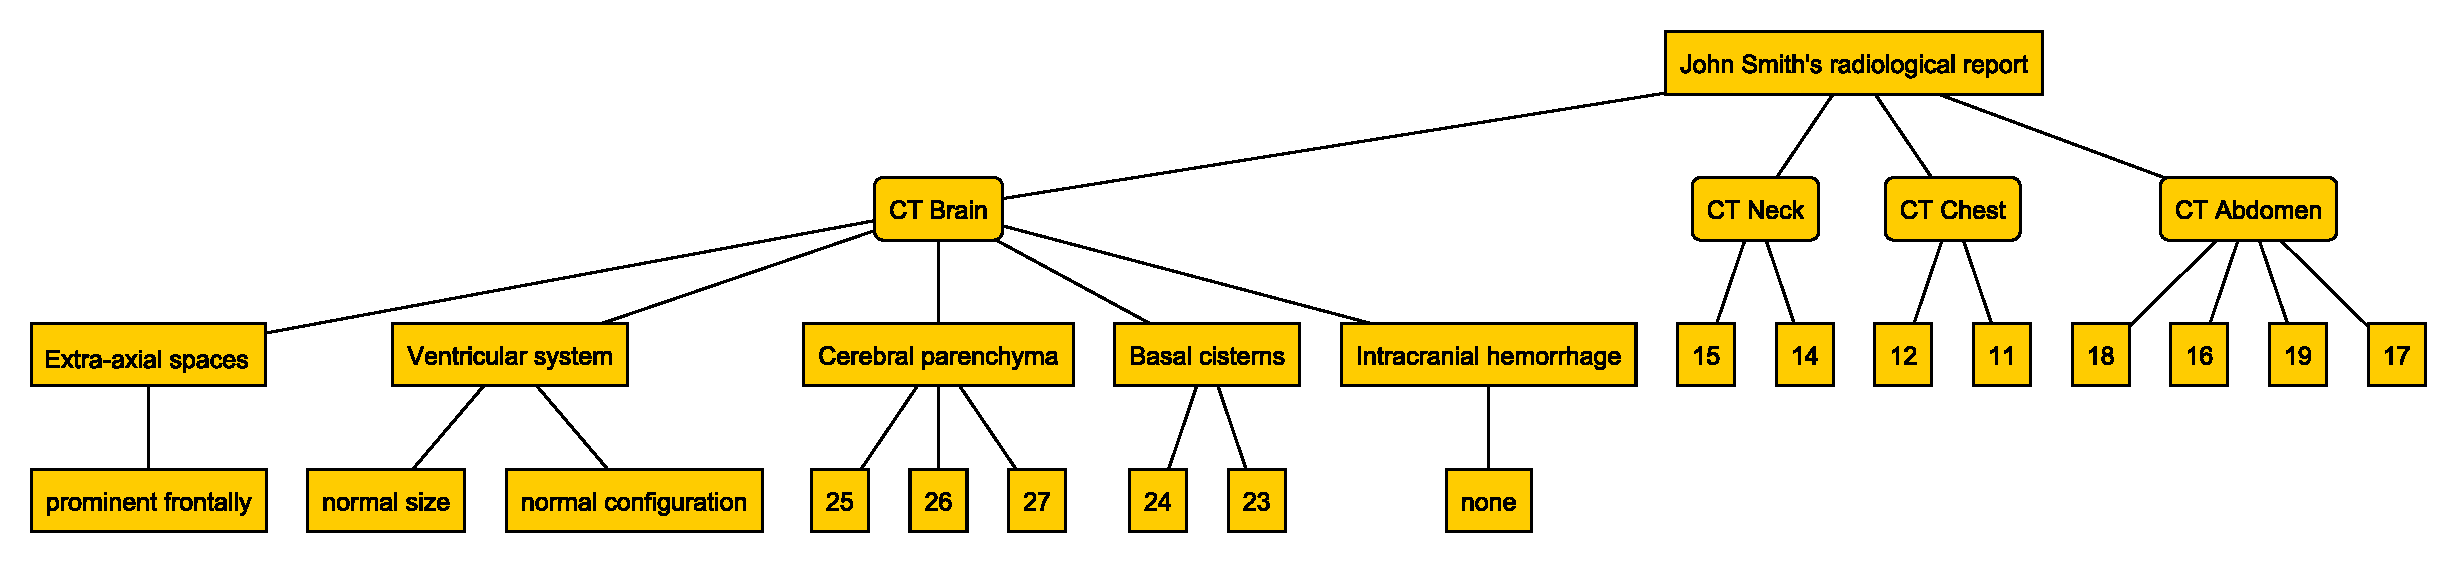
\includegraphics[width=1\linewidth]{../report-tree}
	\label{fig:report-tree}
\end{figure}
\end{frame}

\begin{frame}
\frametitle{Reporting ontology}
\begin{figure}
	\centering
	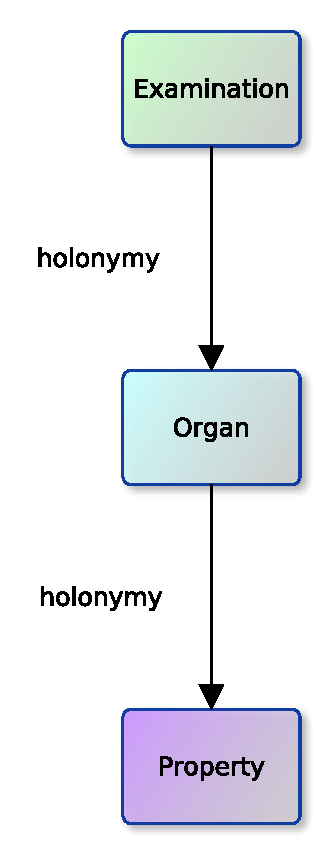
\includegraphics[width=0.2\linewidth]{../report-semantic}
	\caption{Types of entities and relations between them}
	\label{fig:report-ontology}
\end{figure}
\end{frame}




\begin{frame}
\frametitle{Textual representation (simple report)}
\begin{figure}
\centering
\includegraphics[width=\linewidth]{../rendered-report}
\label{fig:rendered-report}
\end{figure}
\end{frame}


\begin{frame}
\frametitle{Textual representation (detailed report using Polish template)}
\begin{figure}
	\centering
	\includegraphics[width=0.68\linewidth]{../rendered-report-pl-bad}
	\label{fig:rendered-report}
\end{figure}
\end{frame}

\begin{frame}
\frametitle{Modified workflow}
\begin{figure}
	\centering
	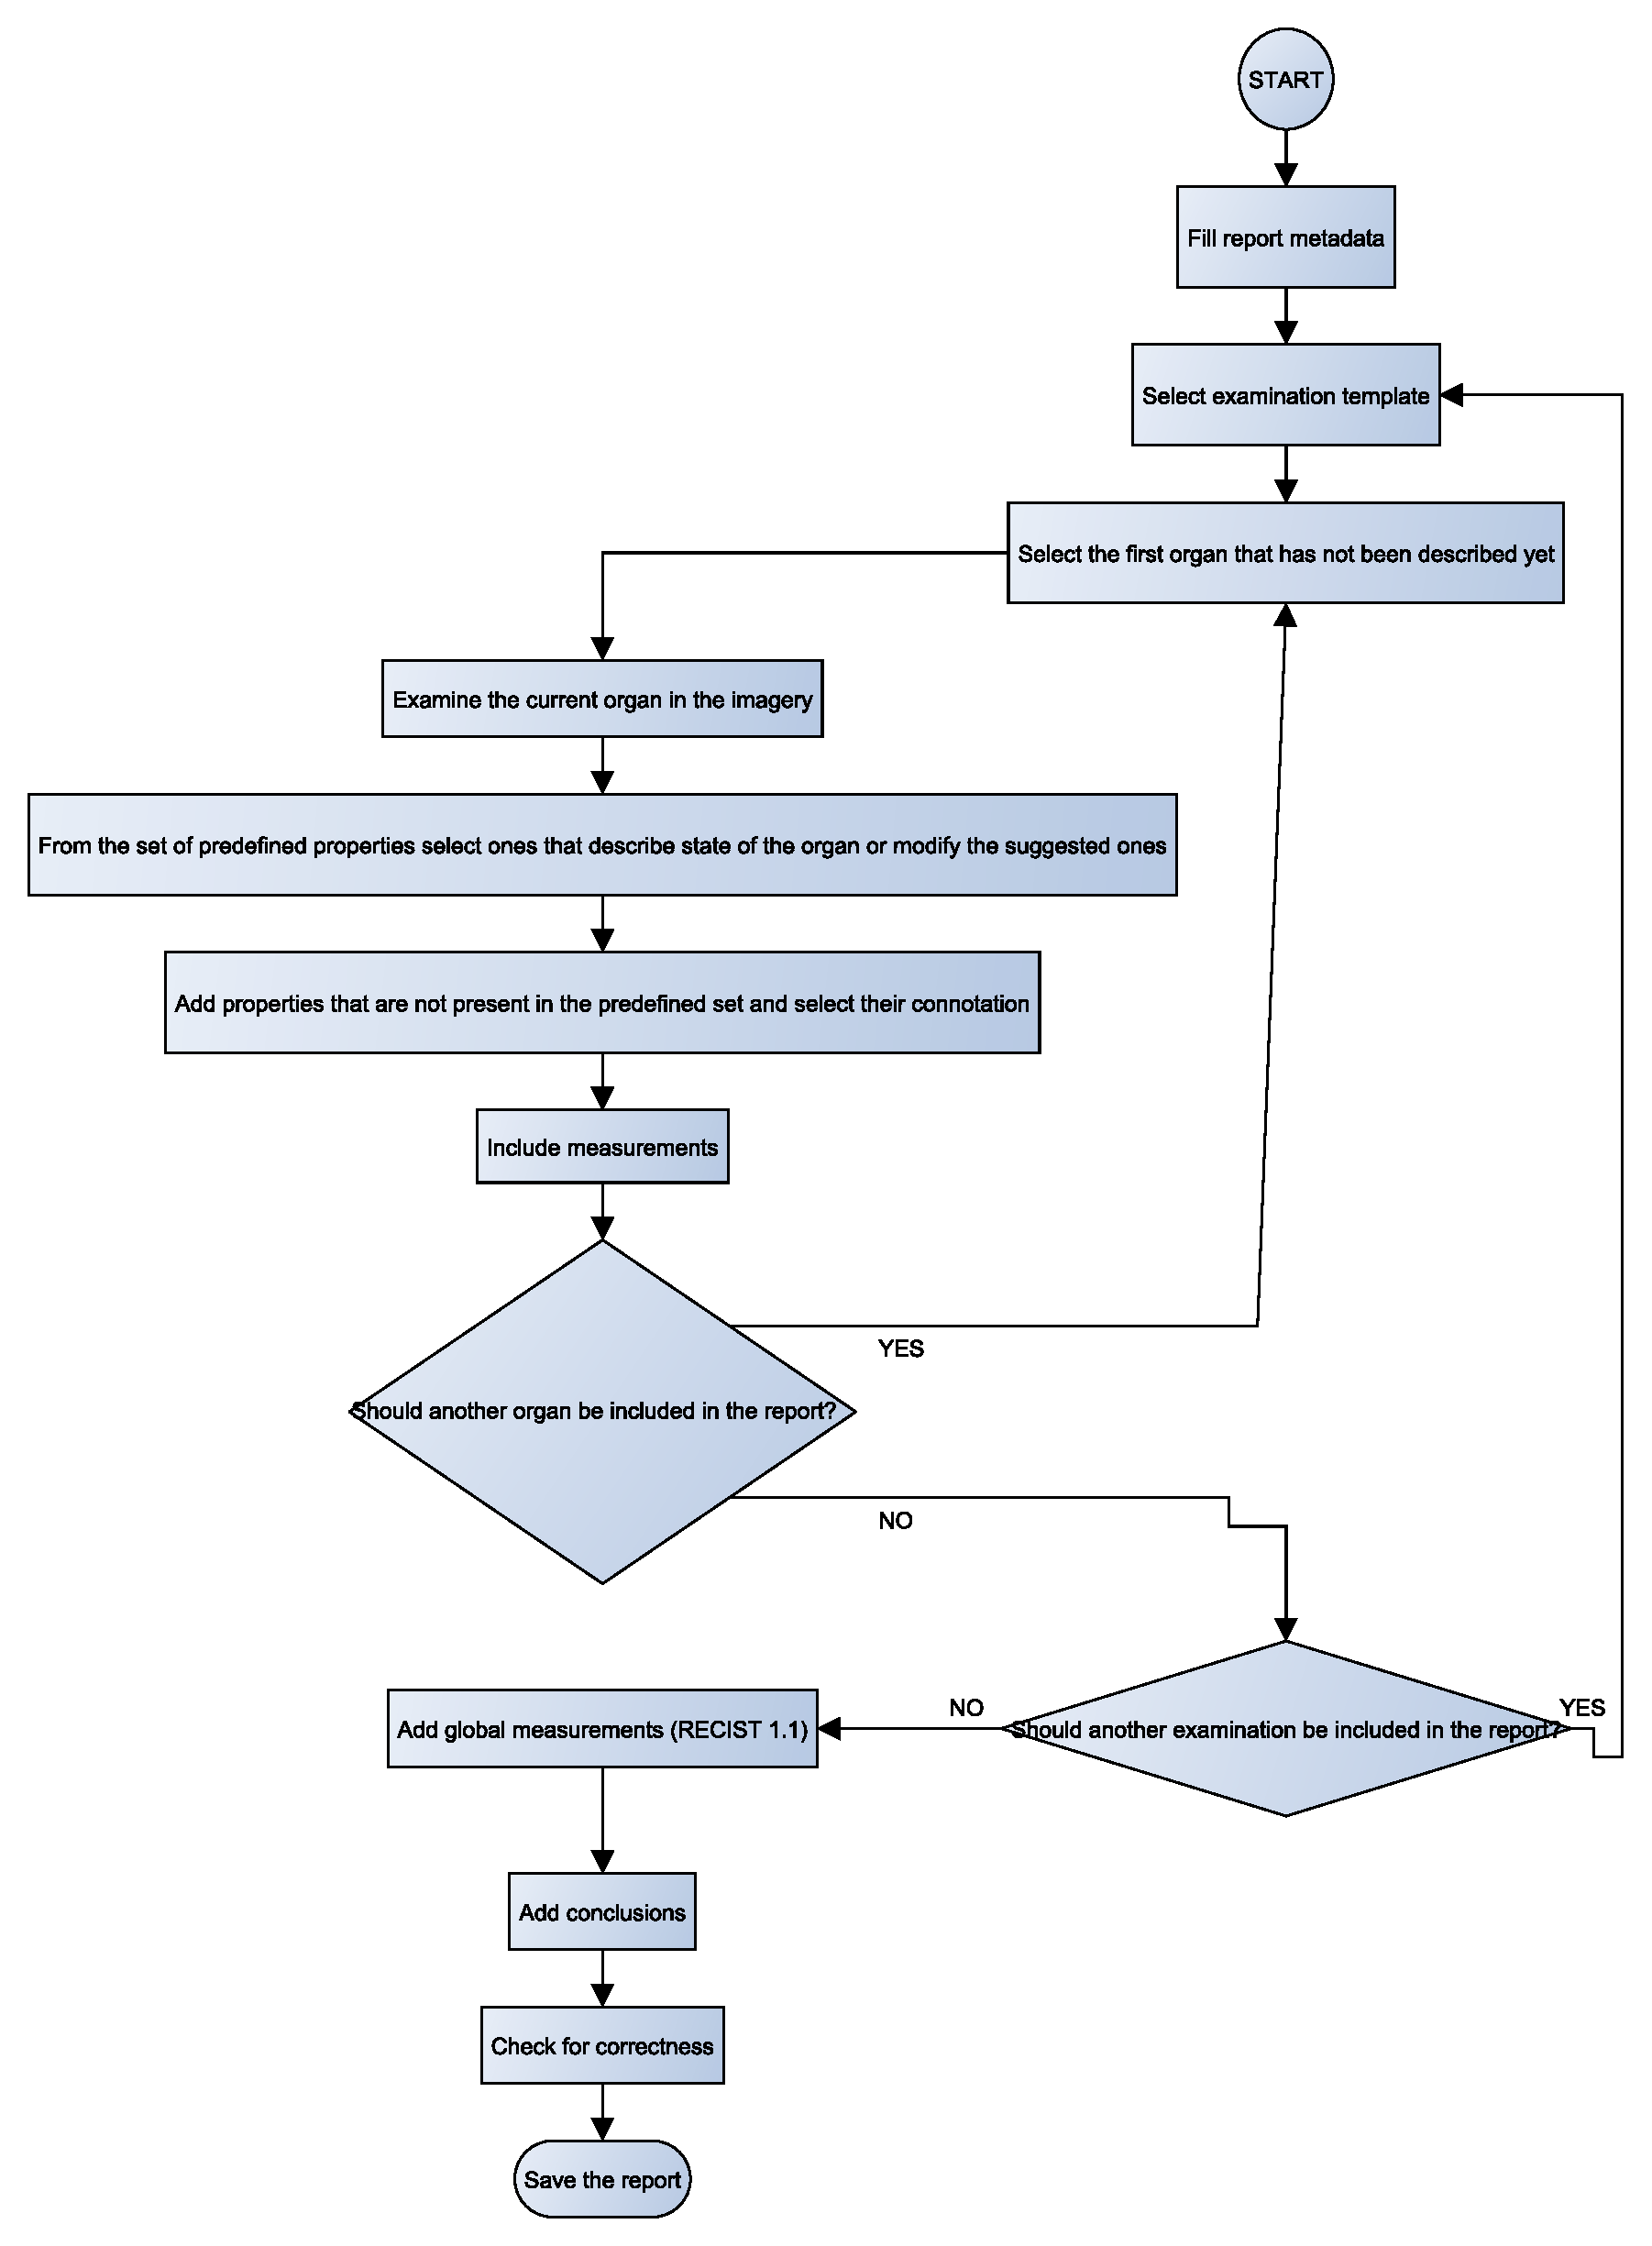
\includegraphics[width=0.5\linewidth]{../report-workflow}
	\label{fig:report-workflow}
\end{figure}
\end{frame}



\subsection{Technological stack}
\begin{frame}
\frametitle{Technological stack}
Web application
\begin{itemize}
	\item backend 
	\begin{itemize}
		\item C\#
		\item ASP.NET
		\item MS SQL 
	\end{itemize}
	\item frontend 
	\begin{itemize}
		\item AngularJS, ES5 
		\item utility modules use ASP.NET + Razor Views
	\end{itemize}
\end{itemize}
\end{frame}

\begin{frame}
\frametitle{System architecture and communication}
\begin{figure}
	\centering
	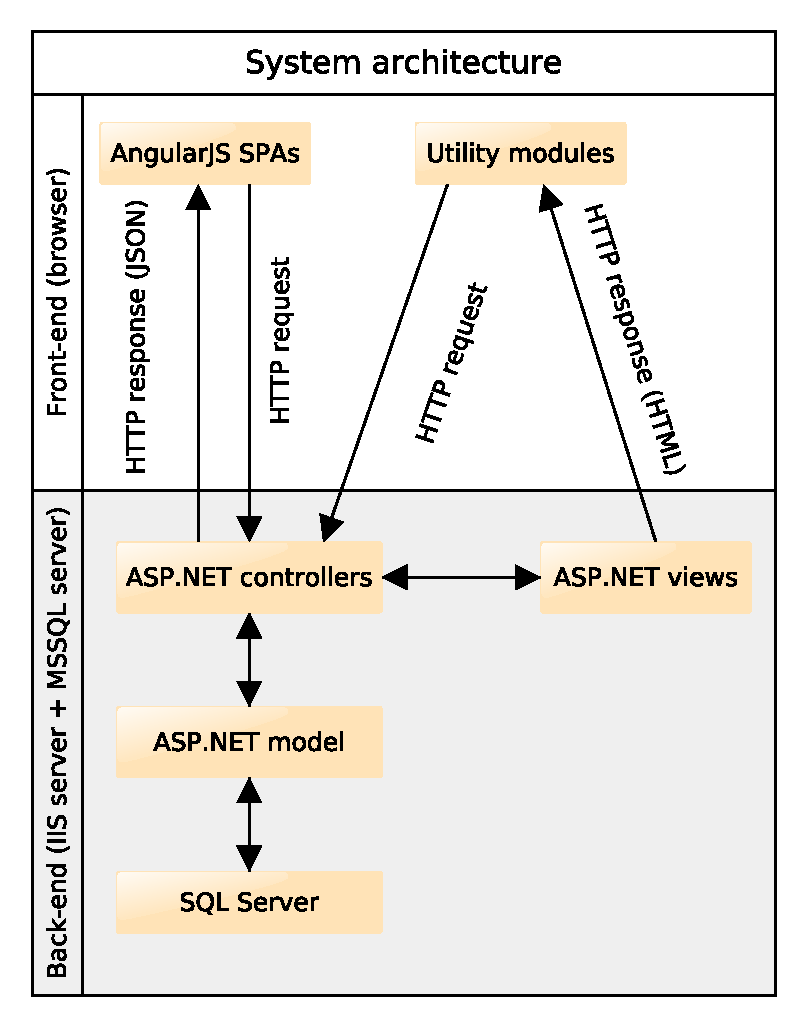
\includegraphics[width=0.6\linewidth]{../architecture}
	\label{fig:rendered-report}
\end{figure}
\end{frame}


\begin{frame}
\frametitle{Report editor interface}
\begin{figure}
	\centering
	\includegraphics[width=1\linewidth]{../examination-list}
	\label{fig:examination-list}
\end{figure}
\end{frame}

\begin{frame}
\frametitle{Organ list}
\begin{figure}
	\centering
	\includegraphics[width=1\linewidth]{../report-organs}
	\label{fig:organ-list}
\end{figure}
\end{frame}

\begin{frame}
\frametitle{Properties}
\begin{figure}
	\centering
	\includegraphics[width=0.8\linewidth]{../properties-modal}
	\label{fig:properties-list}
\end{figure}
\end{frame}



\begin{frame}
\frametitle{Generated report with RECIST 1.1 measurements}
\begin{figure}
	\centering
	\includegraphics[width=1\linewidth]{../report-copy-to-clipboard}
	\label{fig:report-copy-to-clipboard}
\end{figure}
\end{frame}

\section {Validation}

\begin{frame}
\frametitle{Learning curve and productivity improvements}
\begin{figure}
	\centering
	\includegraphics[width=1\linewidth]{productivity_improvements_chart}
\end{figure}
\end{frame}

\begin{frame}
\frametitle{Validation}
Places where the software was used:
\begin{itemize}
	\item Several independent teleradiologists
	\item Small hospital in Wieliszew
	\item Large network of clinics in Łódź
\end{itemize}

Conclusions:
\begin{itemize}
	\item 25 battle-tested templates containing 180 organs
	\item about 1300 reports 
	\item Reports generated about 3 times faster
\end{itemize}
\end{frame}

\begin{frame}
\frametitle{Thanks for your attention}
\end{frame}
\end{document}
